\documentclass[12pt]{article}
\linespread{1}

% margins
\setlength{\textwidth}{6.5in}
\setlength{\textheight}{8.75in}
\setlength{\oddsidemargin}{-0.1in}
\setlength{\topmargin}{-0.1in}
\setlength{\baselineskip}{10pt}

% load packages
\usepackage{amsmath}
\usepackage{amsfonts}
\usepackage{lscape}
\usepackage[round]{natbib}
\usepackage{graphicx}
\graphicspath{{figures_old/}{figures/}{figures_old/roc}{figures_old/calibration_curves}}
\usepackage{amssymb}
\usepackage{color}
\usepackage{hyperref}
\usepackage{booktabs}
\usepackage{verbatim}

% style setup
\bibliographystyle{plainnat}
\pagestyle{empty}
\setlength\parindent{0pt}
\setlength{\parskip}{\baselineskip}

% new commands
\newcommand{\indist}{\overset{d}{\rightarrow}}
\newcommand{\inprob}{\overset{P}{\rightarrow}}
\newcommand{\tabby}{\hspace{10pt}}
\newcommand{\ones}{{\bf 1}}
\newcommand{\tp}{\intercal}
\newcommand{\iprod}[2]{\langle #1 , #2 \rangle}

\newcommand{\note}[1]{\textcolor{red}{#1}}

% header
\title{HOSEA Aim I -- Report}
\author{Simon Fontaine}
\date{\today}

\begin{document}

\maketitle

\clearpage
\newpage
\section*{Calibration \& threshold}


\begin{minipage}{0.5\textwidth}\small
\begin{tabular}{rccc}
\toprule
\textbf{Threshold} & \textbf{TPR} 
& \textbf{PPV} & \textbf{Det. prev.} \\
\midrule

    10 & 99.51 & 0.14 & 79.20 \\ 
    15 & 99.19 & 0.14 & 76.68 \\ 
    20 & 99.05 & 0.15 & 74.69 \\ 
    25 & 98.74 & 0.15 & 72.82 \\ 
    30 & 98.46 & 0.15 & 70.91 \\ \addlinespace
    35 & 97.93 & 0.16 & 68.92 \\ 
    40 & 97.26 & 0.16 & 66.88 \\ 
    45 & 96.77 & 0.17 & 64.81 \\ 
    50 & 95.82 & 0.17 & 62.74 \\ 
    55 & 94.66 & 0.17 & 60.67 \\ \addlinespace 
    60 & 93.86 & 0.18 & 58.59 \\ 
    65 & 92.80 & 0.18 & 56.51 \\ 
    70 & 91.54 & 0.19 & 54.44 \\ 
    75 & 89.93 & 0.19 & 52.41 \\ 
    80 & 88.77 & 0.20 & 50.40 \\  \addlinespace
    85 & 87.40 & 0.20 & 48.42 \\ 
    90 & 86.03 & 0.21 & 46.47 \\ 
    95 & 84.35 & 0.21 & 44.57 \\ 
   100 & 82.91 & 0.22 & 42.70 \\ 
   105 & 80.84 & 0.22 & 40.87 \\  \addlinespace
   110 & 79.26 & 0.23 & 39.08 \\ 
   115 & 77.89 & 0.23 & 37.35 \\ 
   120 & 76.06 & 0.24 & 35.67 \\ 
   125 & 74.34 & 0.24 & 34.03 \\ 
   130 & 72.27 & 0.25 & 32.44 \\  \addlinespace
   135 & 69.95 & 0.25 & 30.91 \\ 
   140 & 68.30 & 0.26 & 29.46 \\ 
   145 & 66.34 & 0.26 & 28.06 \\ 
   150 & 64.41 & 0.27 & 26.71 \\
   155 & 62.97 & 0.27 & 25.44 \\  \addlinespace
   160 & 61.21 & 0.28 & 24.21 \\ 
   165 & 59.39 & 0.29 & 23.05 \\ 
   170 & 57.63 & 0.29 & 21.94 \\ 
   175 & 55.70 & 0.30 & 20.88 \\
   180 & 53.88 & 0.30 & 19.89 \\  \addlinespace
   185 & 52.61 & 0.31 & 18.93 \\ 
   190 & 50.97 & 0.31 & 18.02 \\ 
   195 & 49.49 & 0.32 & 17.17 \\ 

\bottomrule
\end{tabular}

\end{minipage} \hfill
\begin{minipage}{0.5\textwidth}\small
\begin{tabular}{rccc}
\toprule
\textbf{Threshold} & \textbf{TPR} 
& \textbf{PPV} & \textbf{Det. prev.} \\
\midrule 
   200 & 47.81 & 0.32 & 16.36 \\ 
   210 & 45.03 & 0.34 & 14.88 \\ 
   220 & 41.84 & 0.34 & 13.53 \\ 
   230 & 39.35 & 0.35 & 12.34 \\ 
   240 & 36.96 & 0.36 & 11.25 \\  \addlinespace
   250 & 34.85 & 0.38 & 10.28 \\ 
   260 & 32.82 & 0.39 & 9.40 \\ 
   270 & 31.52 & 0.41 & 8.62 \\ 
   280 & 29.52 & 0.41 & 7.91 \\ 
   290 & 27.87 & 0.43 & 7.26 \\  \addlinespace
   300 & 26.04 & 0.43 & 6.67 \\ 
   325 & 22.01 & 0.45 & 5.43 \\ 
   350 & 18.67 & 0.46 & 4.46 \\ 
   375 & 16.15 & 0.49 & 3.66 \\ 
   400 & 14.04 & 0.51 & 3.03 \\  \addlinespace
   425 & 12.57 & 0.55 & 2.52 \\ 
   450 & 10.74 & 0.57 & 2.10 \\ 
   475 & 9.23 & 0.58 & 1.76 \\ 
   500 & 8.11 & 0.61 & 1.47 \\ 
   600 & 4.32 & 0.64 & 0.75 \\  \addlinespace
   700 & 2.81 & 0.79 & 0.39 \\ 
   800 & 1.76 & 0.90 & 0.22 \\ 
   900 & 1.02 & 0.92 & 0.12 \\ 
  1000 & 0.49 & 0.79 & 0.07 \\ 
  1100 & 0.28 & 0.74 & 0.04 \\  \addlinespace
  1200 & 0.18 & 0.73 & 0.03 \\ 
  1300 & 0.07 & 0.50 & 0.02 \\ 
  1400 & 0.07 & 0.81 & 0.01 \\ 
  1500 & 0.07 & 1.18 & 0.01 \\ 
  1600 & 0.04 & 0.90 & 0.00 \\  \addlinespace
  1700 & 0.04 & 1.33 & 0.00 \\ 
  1800 & 0.04 & 2.00 & 0.00 \\ 
  1900 & 0.04 & 2.94 & 0.00 \\ 
  2000 & 0.04 & 4.00 & 0.00 \\ \\ \addlinespace \\ \\ \\
\bottomrule
\end{tabular}

\end{minipage}




\begin{figure}[h]
\centering
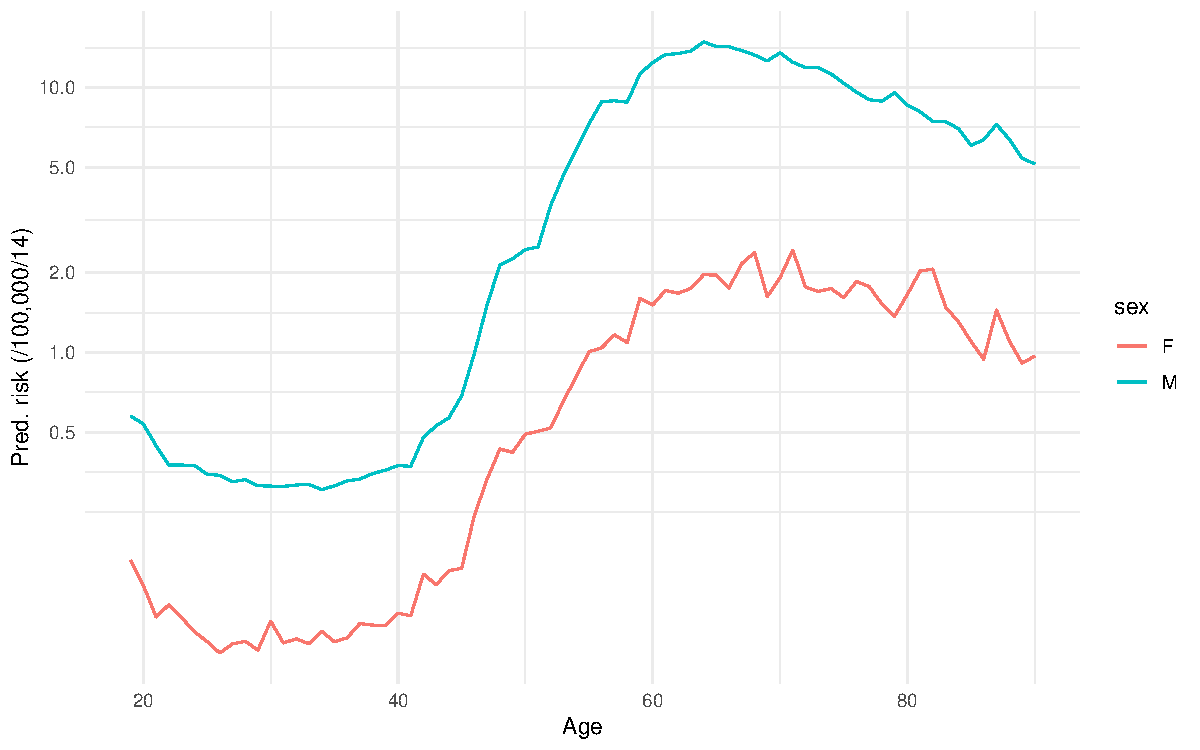
\includegraphics[width=\textwidth]{figures/risk_age_sex14.pdf}
\caption{The average annalized risk is 7.6/100,000: for males, it is 8.2/100,000 and, for females, it is 0.7/100,000. }

\end{figure}



\begin{figure}[h]
\centering
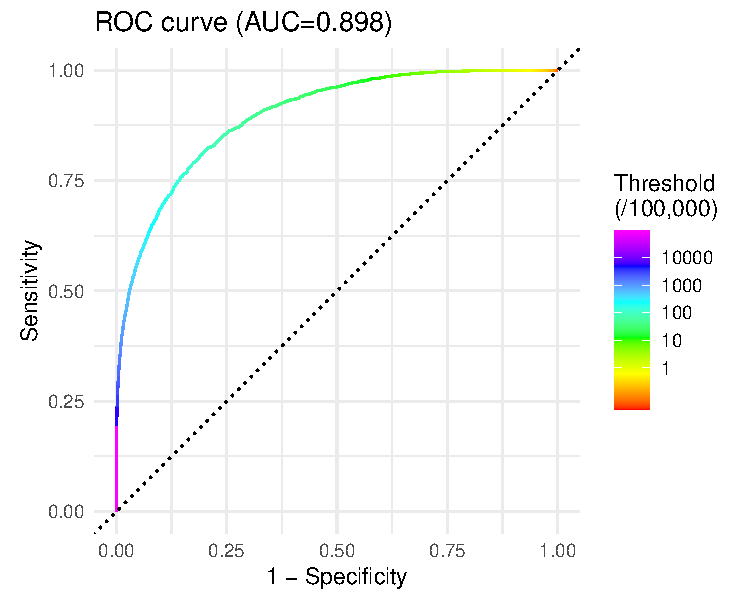
\includegraphics[width=\textwidth]{figures/roc.pdf}

\end{figure}



\begin{figure}[h]
\centering
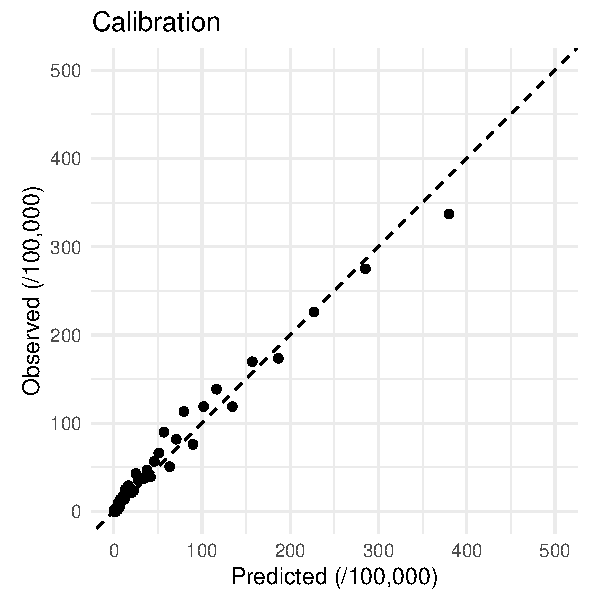
\includegraphics[width=0.6\textwidth]{figures/calibration50_all_zoom.pdf}
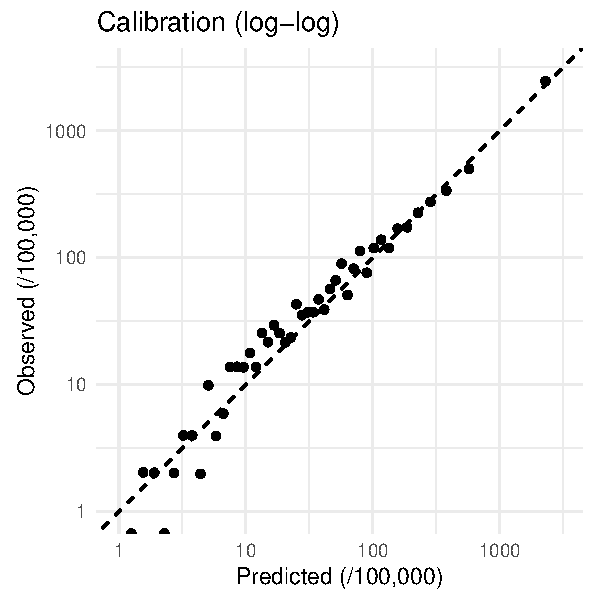
\includegraphics[width=0.6\textwidth]{figures/calibration50_all_log.pdf} \\
Each point represent 2\% of the test data, split using predicted risk quantiles. The top plot is cropped on the right and top
 so we can focus on the more important region. HL test: "H=49.8507485754787, df=49, p=0.439294514740096"

\end{figure}


\clearpage
\section*{Comparison}


For these comparisons:
\begin{itemize}
\item Subset to test observations
\item Filter out patients with missing information for HUNT/Kunzmann/Guidelines
\item i.e., require age, BMI, race, smoking status, gerd, h2r/ppi
\item 407K patients, 1192 cases (292/100,000)
\item AUC + 95\% CI using DeLong method
\end{itemize}

\begin{figure}[h]
\centering
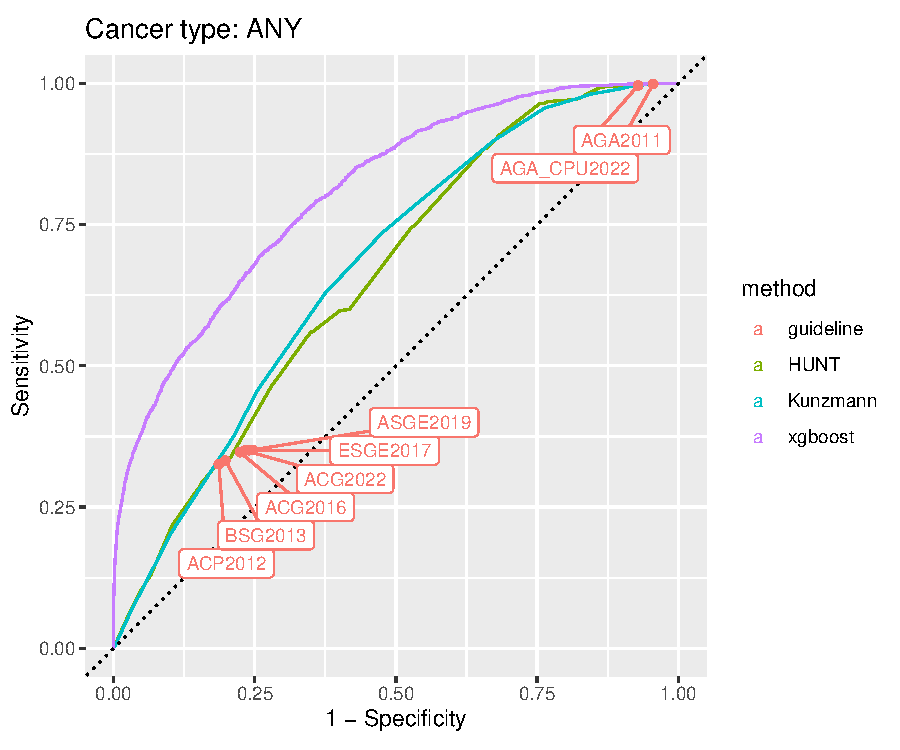
\includegraphics[width=1.0\textwidth]{figures/comparison_ANY.pdf}
\end{figure}

\begin{figure}[h]
\centering
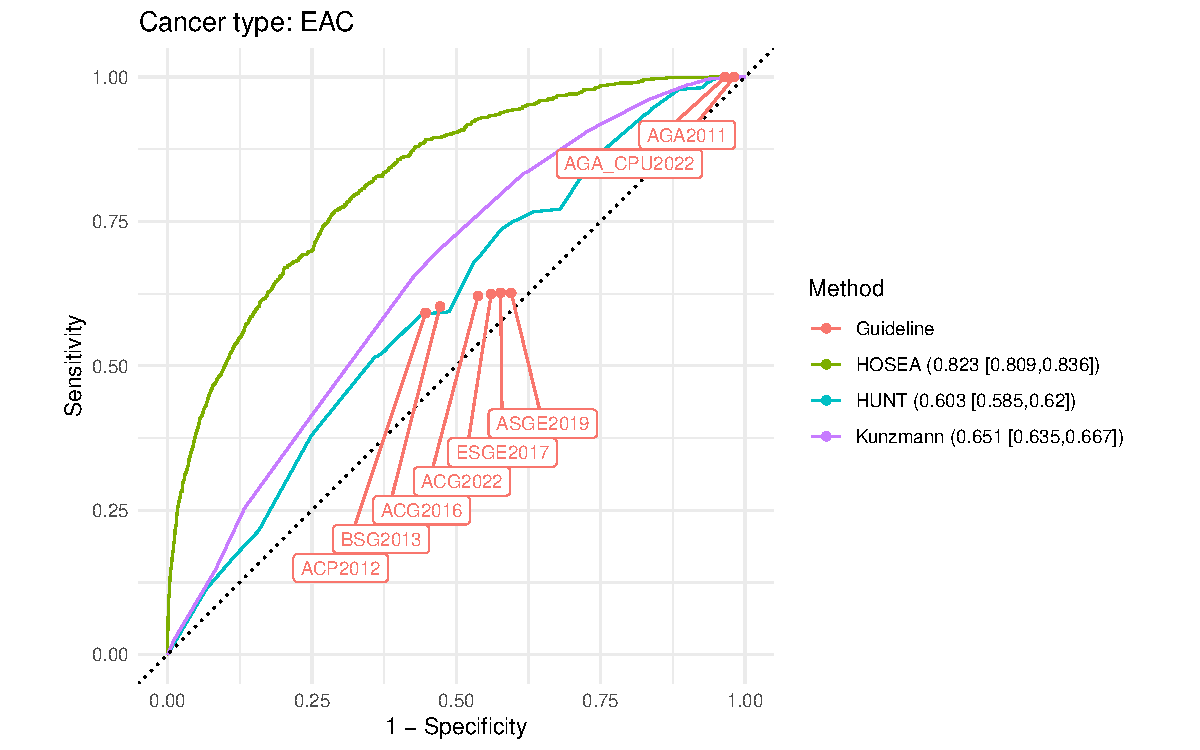
\includegraphics[width=1.0\textwidth]{figures/comparison_EAC.pdf}
\end{figure}

\begin{figure}[h]
\centering
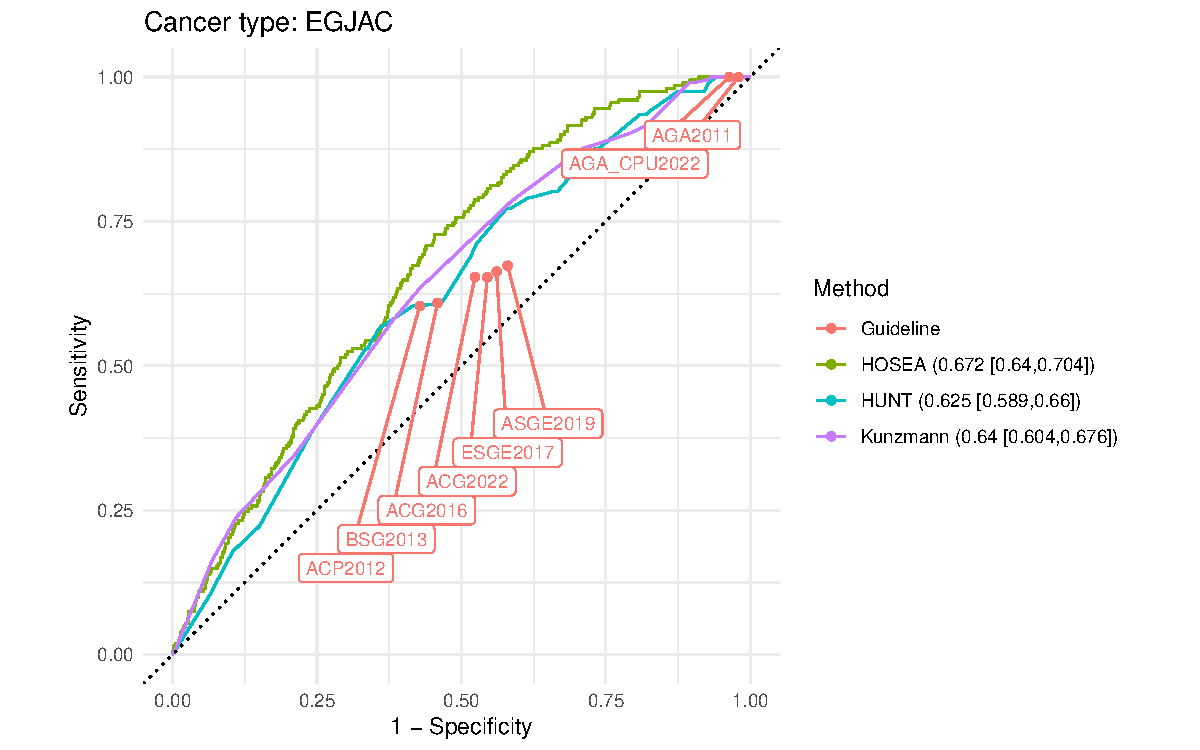
\includegraphics[width=1.0\textwidth]{figures/comparison_EGJAC.pdf}
\end{figure}

\clearpage

\begin{center}
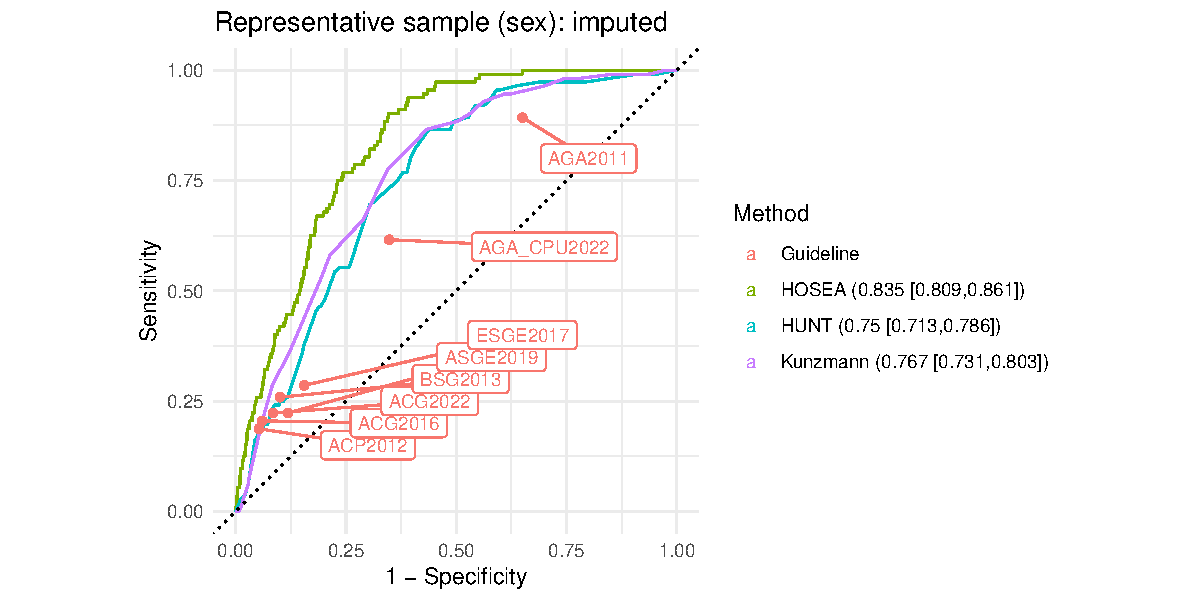
\includegraphics[width=1.0\textwidth]{figures/comparison_sex_imputed.pdf}
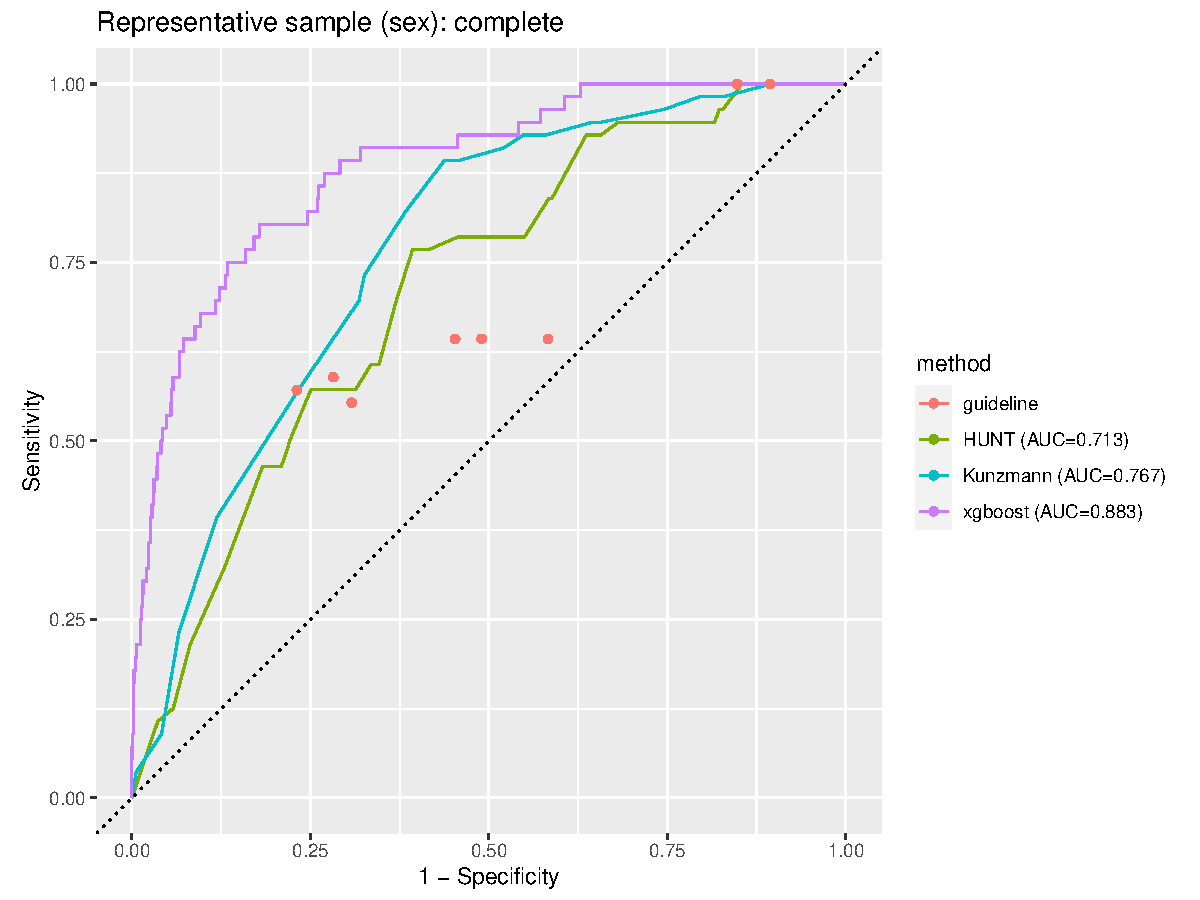
\includegraphics[width=1.0\textwidth]{figures/comparison_sex_complete.pdf}
\end{center}



\clearpage

\section*{Gain Variable importance}

``Gain represents fractional contribution of each feature to the model based on the total gain of this feature's splits. 
Higher percentage means a more important predictive feature.''

Some notes:
\begin{itemize}
\item These are additive, so we can compute the importance of a group of features.
\item They sum up to 1
\item We can only look at the relationship with the feature value (e.g., mostly positive, mostly negative) for single features
\end{itemize}

\begin{center}
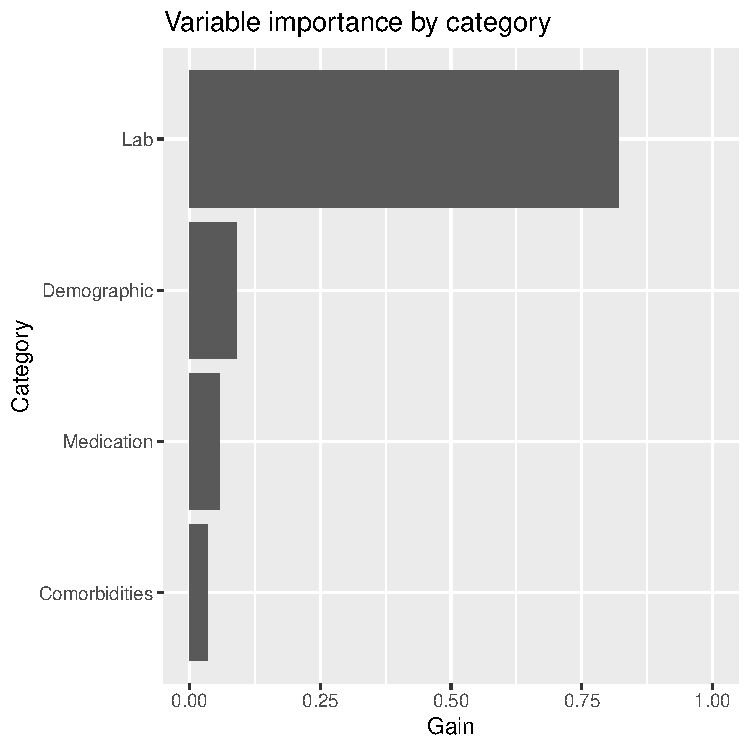
\includegraphics[width=0.6\textwidth]{figures/pdp_new/vi_cat.pdf}
\end{center}
\begin{center}
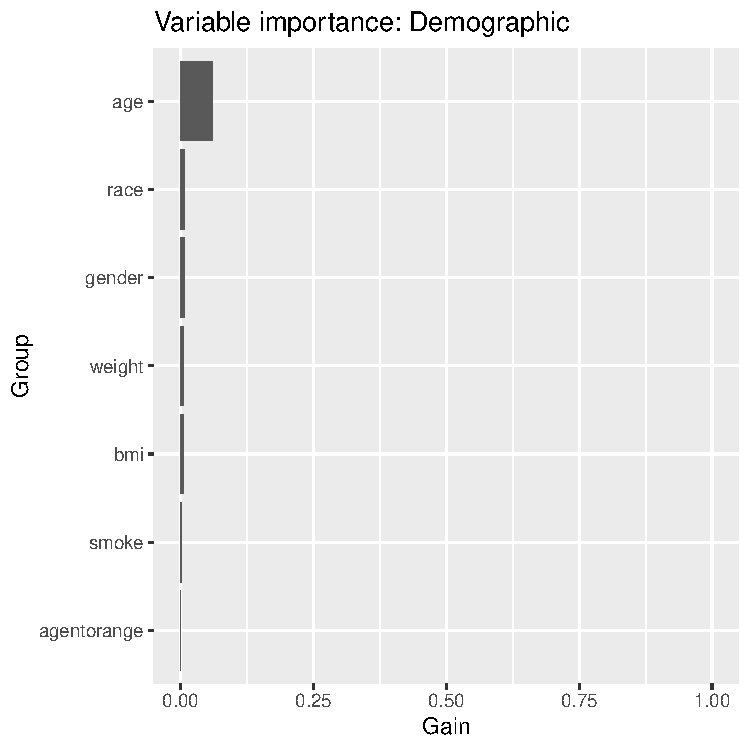
\includegraphics[width=0.6\textwidth]{figures/pdp_new/vi_group_Demographic.pdf}
\end{center}
\begin{center}
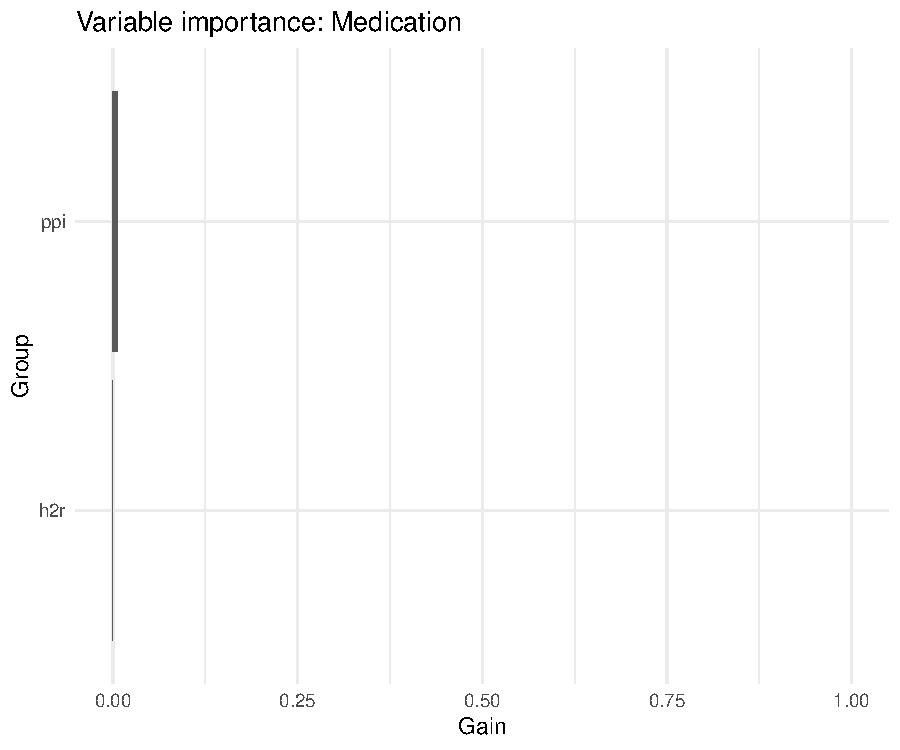
\includegraphics[width=0.6\textwidth]{figures/pdp_new/vi_group_Medication.pdf}
\end{center}
\begin{center}
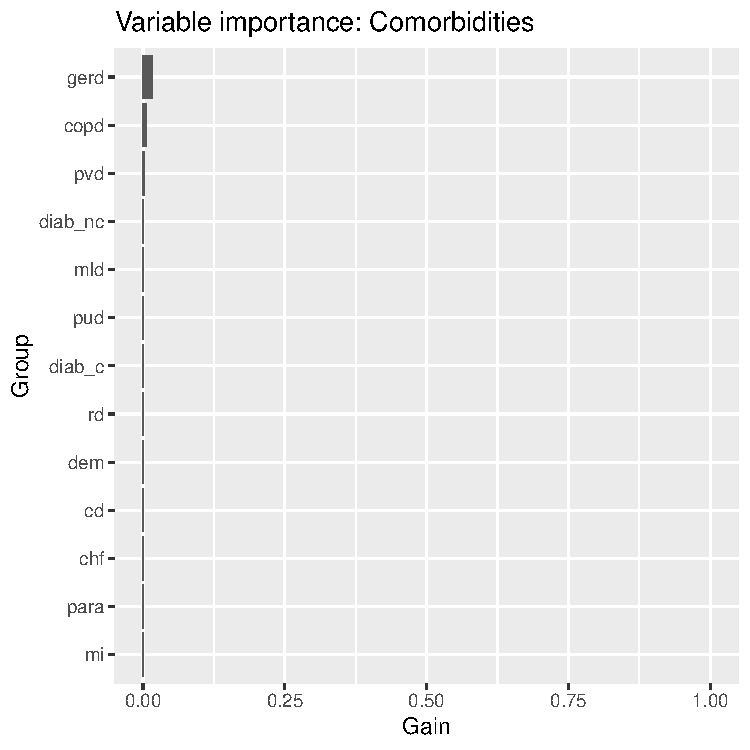
\includegraphics[width=0.6\textwidth]{figures/pdp_new/vi_group_Comorbidities.pdf}
\end{center}
\begin{center}
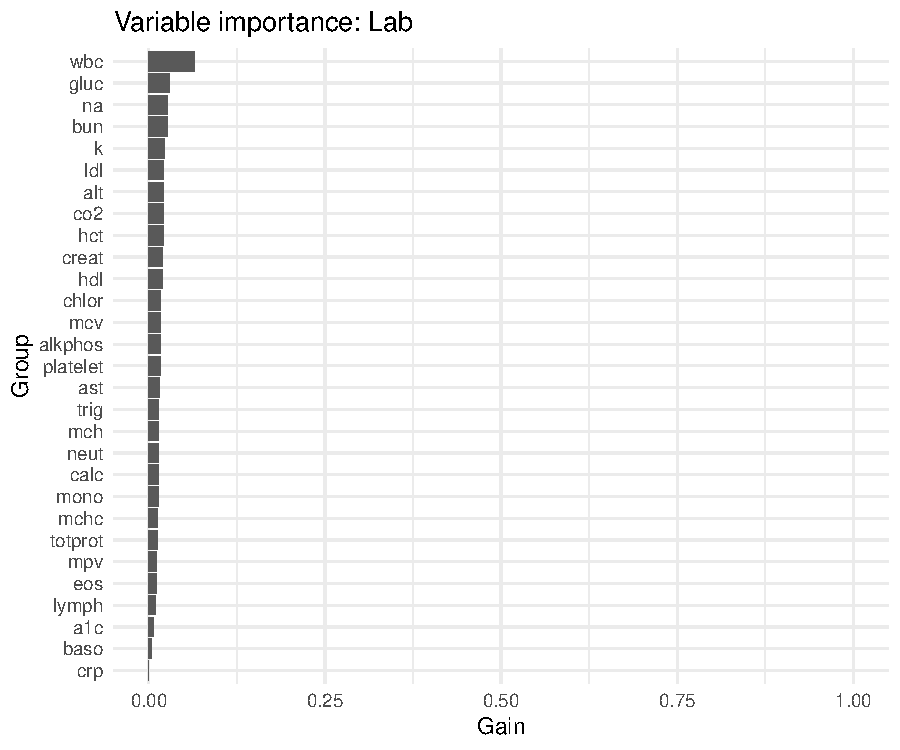
\includegraphics[width=0.6\textwidth]{figures/pdp_new/vi_group_Lab.pdf}
\end{center}

\clearpage

\section*{SHAP Variable Importance}

\begin{itemize}
\item As Gain, this is  additive, but does not sum to 1
\item Local measure, can be aggreagted using mean absolute value 
\item Understood as change in log-odds due to this variable (``Given the current set of feature values, 
the contribution of a feature value to the difference between the actual prediction and the mean prediction is the estimated Shapley value.'')
\item Scale to be inderstood as $\beta_jx_{ij}$ in logistic regression $$\text{logit}P[Y_i=1] = \beta_0 + \beta_1x_{i1} + \cdots \beta_px_{ip}$$
\end{itemize}

\begin{figure}[h]
\centering
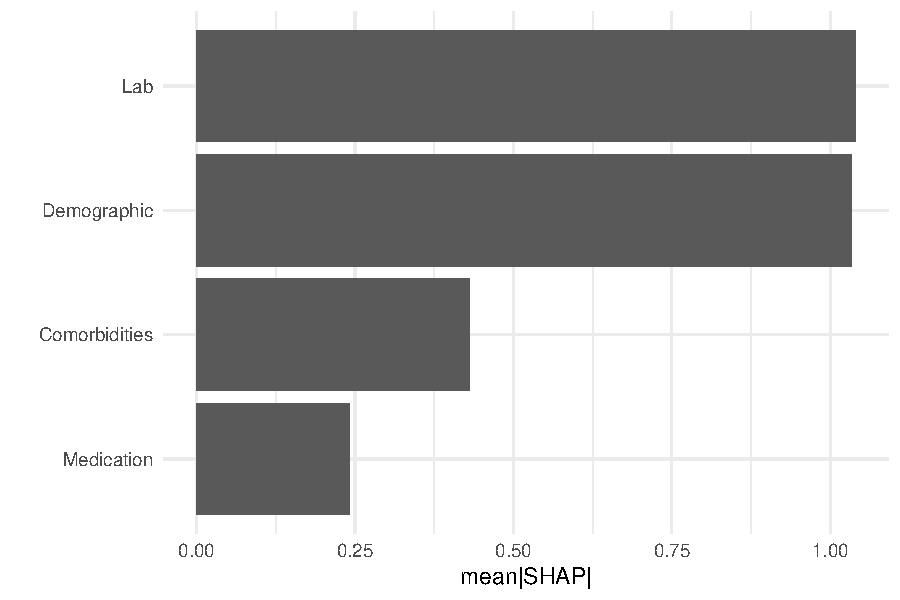
\includegraphics[width=0.6\textwidth]{figures/shap_new/shap_categories.pdf}
\caption{This has mean updated using a representative sample; previously, I was using a sample that over represented cases
so age was much less important.}
\end{figure}
\begin{figure}[h]
\centering
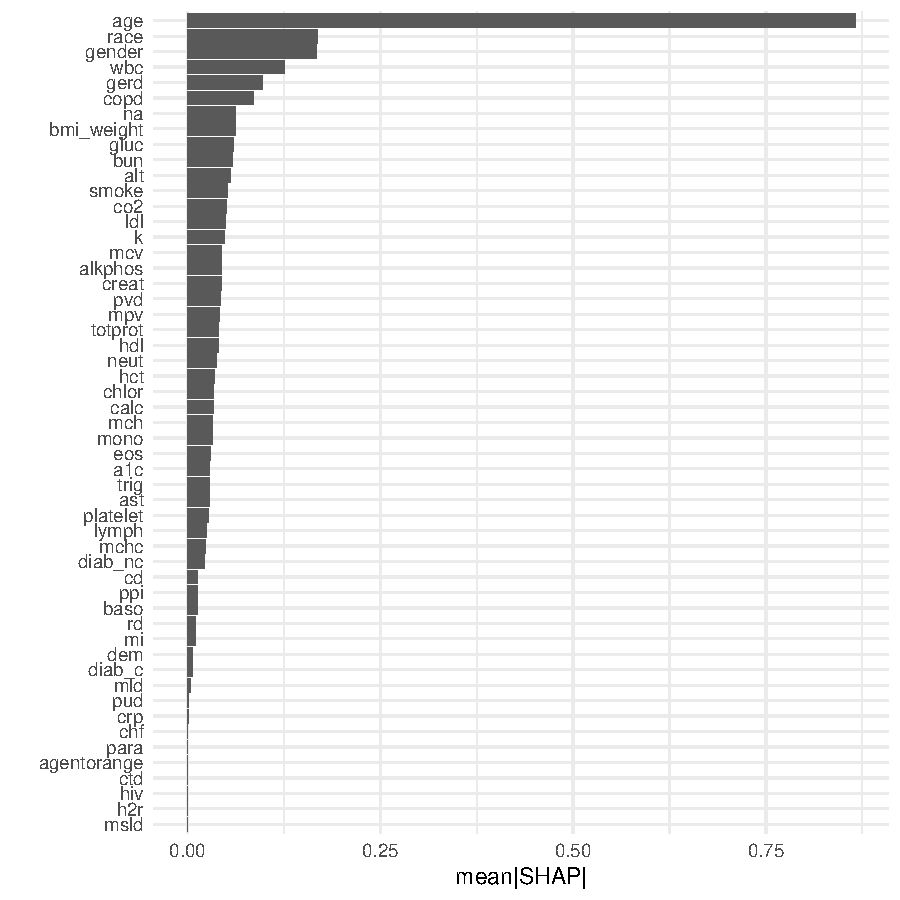
\includegraphics[width=0.96\textwidth]{figures/shap_new/shap_groups.pdf}
\end{figure}
\begin{figure}[h]
\centering
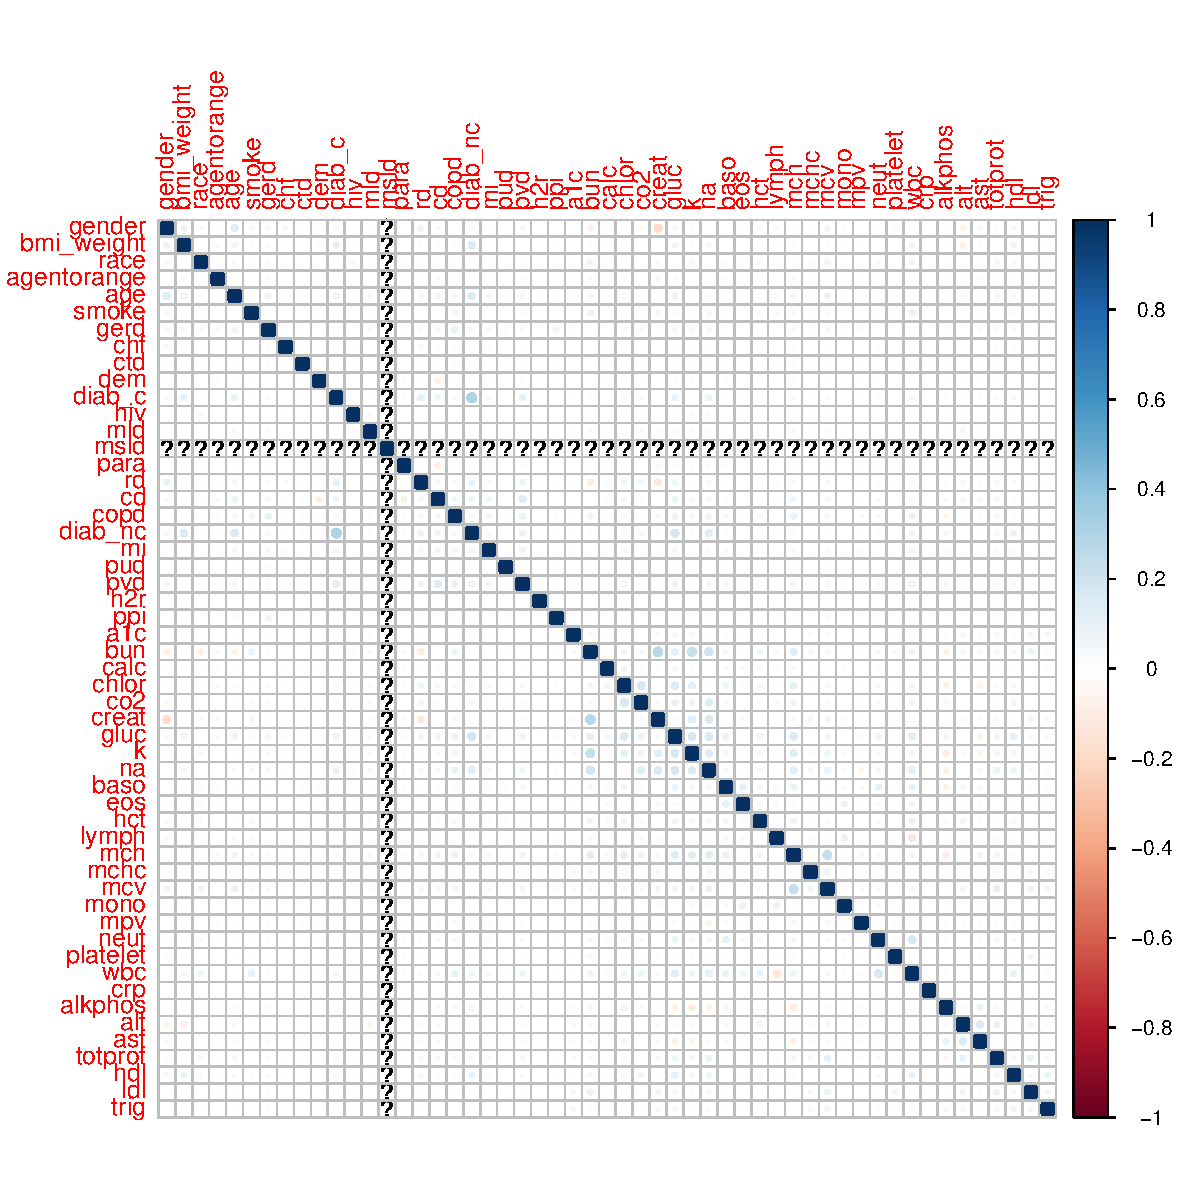
\includegraphics[width=0.96\textwidth]{figures/shap_new/shap_corr.pdf}
\caption{Correlation between group-level Shapley values. Largest absolute correlation in the following table. If two Shapley values
are highly correlated, that means the underlying variables contribute essentially in the same way to the prediction and are therefore redundant.}
\end{figure}

\clearpage
\begin{table}[h]
\centering
\begin{tabular}{llr}
\toprule
\multicolumn{2}{l}{Feature pair} & SHAP correlation \\
\midrule
diab\_c & diab\_nc & 0.31 \\ 
bun & creat & 0.28 \\ 
bun & k & 0.24 \\ 
mch & mcv & 0.23 \\ 
bun & na & 0.19 \\ \addlinespace
gender & creat & -0.18 \\ 
diab\_nc & gluc & 0.18 \\ 
chlor & co2 & 0.17 \\ 
gluc & k & 0.17 \\ 
neut & wbc & 0.17 \\ \addlinespace
gluc & na & 0.17 \\ 
creat & na & 0.16 \\ 
age & diab\_nc & 0.16 \\ 
chlor & gluc & 0.15 \\ 
bmi\_weight & diab\_nc & 0.15 \\ \addlinespace
alt & ast & 0.15 \\ 
k & na & 0.14 \\ 
gluc & mch & 0.14 \\ 
gender & age & 0.14 \\ 
cd & pvd & 0.14 \\  
\bottomrule
\end{tabular}
\caption{Since the largest Shapley correaltion is fairly low, we can be reassured we do not have redundant variables.}
\end{table}


\clearpage
\section*{Identity groups}

\begin{center}
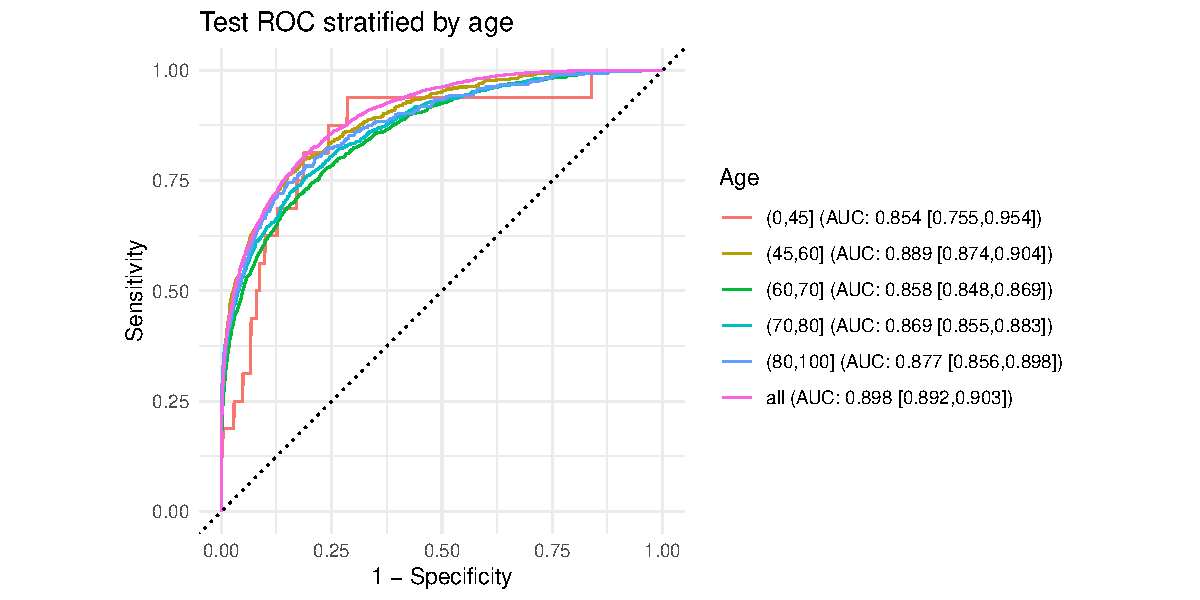
\includegraphics[width=\textwidth]{figures/roc_age.pdf}
\end{center}

\begin{center}
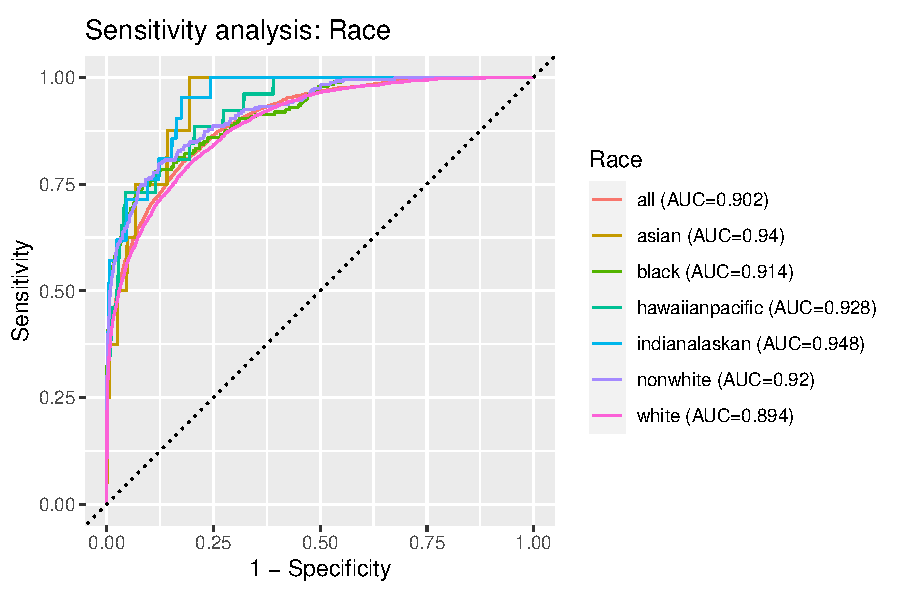
\includegraphics[width=\textwidth]{figures/roc_Race.pdf}
\end{center}

\begin{center}
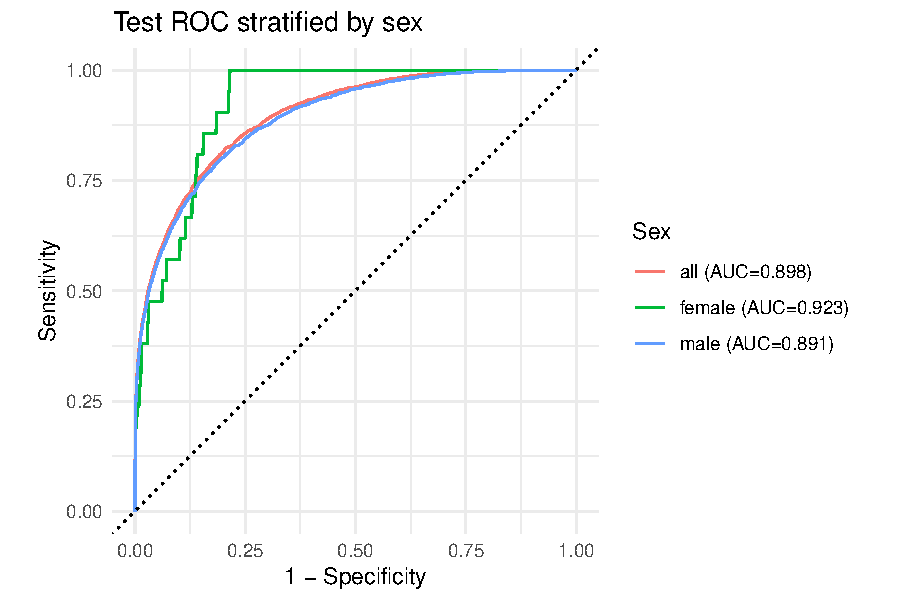
\includegraphics[width=\textwidth]{figures/roc_gender.pdf}
\end{center}



\clearpage
\newpage
\newpage
\newpage


\clearpage
\section*{Cancer stage}

\begin{table}[ht]
\centering
\begin{tabular}{lrr}
  \toprule
 Stage & Test. AUC & Nb. cases \\ 
  \midrule
Any & 0.773 [0.765,0.78] & 2810 \\ \addlinespace
  I & 0.795 [0.773,0.817] & 298 \\ 
  II & 0.798 [0.774,0.822] & 240 \\ 
  III & 0.772 [0.757,0.787] & 631 \\ 
  IV & 0.767 [0.755,0.778] & 1041 \\  \addlinespace
  I+ & 0.775 [0.767,0.783] & 2254 \\ 
  II+ & 0.772 [0.764,0.78] & 1956 \\ 
  III+ & 0.768 [0.759,0.777] & 1716 \\ 
  IV+ & 0.767 [0.755,0.778] & 1041 \\ 
   \bottomrule
\end{tabular}
\caption{Interestingly, it seems slightly harder to predict late stages?}
\end{table}

\begin{figure}[h]
\centering
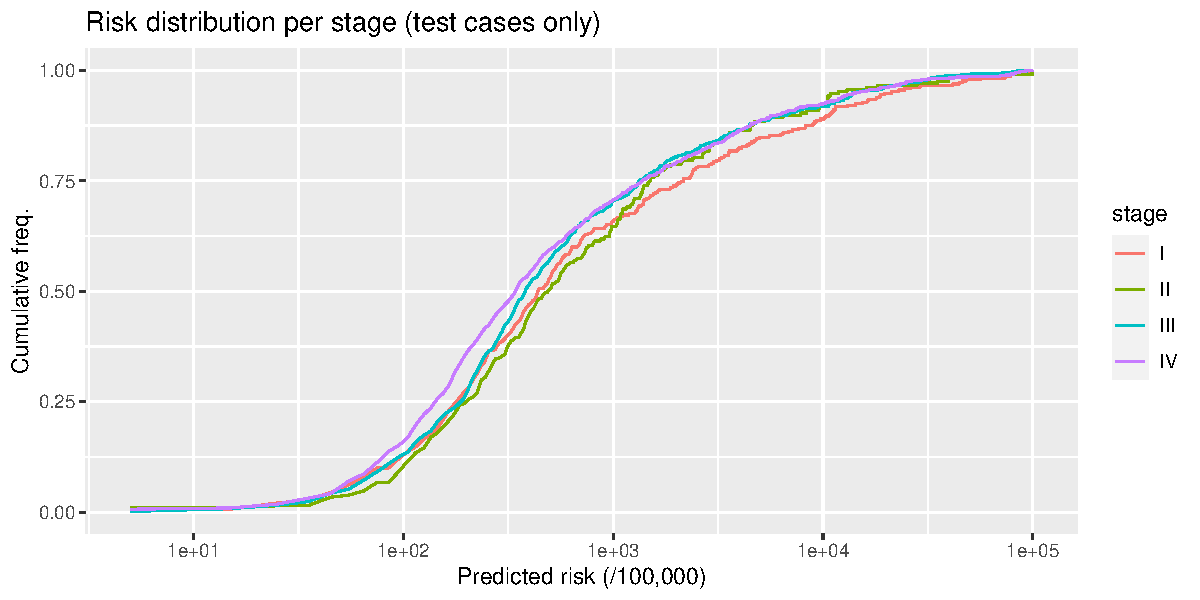
\includegraphics[width=1.0\textwidth]{figures/risk_stage.pdf}
\end{figure}



%
%\clearpage
%\section*{Lab variables interpretation}
%
%\begin{itemize}
%\item I started to look at ways we could interpret the effect of the lab variables on the predictions
%\item I focused on \texttt{mch} for now to develop the approach
%\item During this, I noticed that the labels for maxdiff and mindiff were flipped ... This doesn't change anything about performance though.
%\item same thing for min and max ...
%%\item Some important fact is that when tv is 0, maxdiff (mindiff) is negative or mindiff (maxdiff) is positive, that means there are just a few observations
%%since random variations trhough any signal should occur. This means any switch around these points indicate that the model is mostly learning 
%%that the patient had few observations for that variable ...
%%\item Maybe we should require, say, 5 observations for tv, mindiff, maxdiff? Should we include meandiff to get the overall trend?
%\end{itemize}
%
%\begin{figure}[h]
%\centering
%\includegraphics[width=1.0\textwidth]{figures/shap_new/shap_lab_mch.pdf}
%\caption{SHAP values for a sample with overrepresentation of cases ranked according to \texttt{mean|SHAP|} from top 
%to bottom.}
%\end{figure}
%
%\begin{figure}[h]
%\centering
%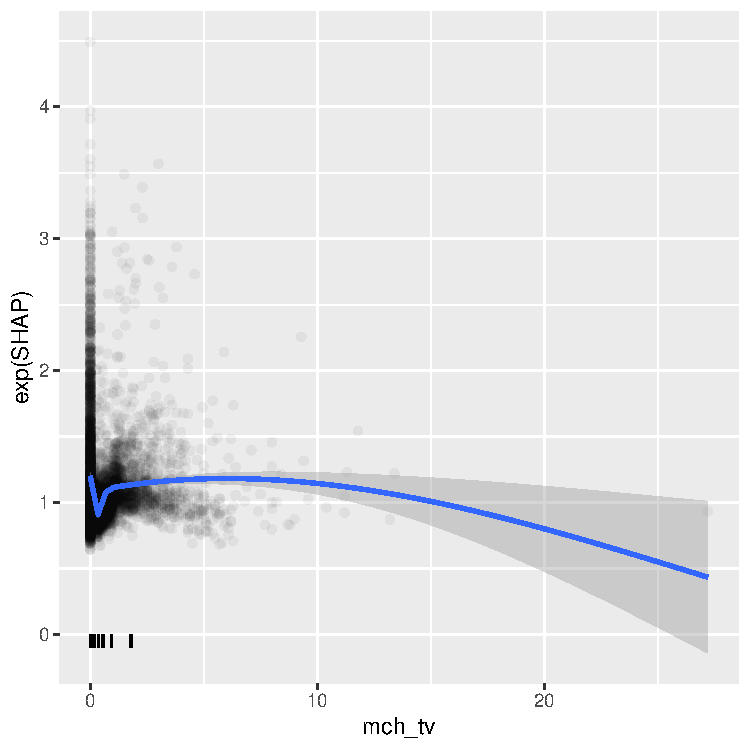
\includegraphics[width=0.49\textwidth]{figures/shap_new/mch_tv.pdf}
%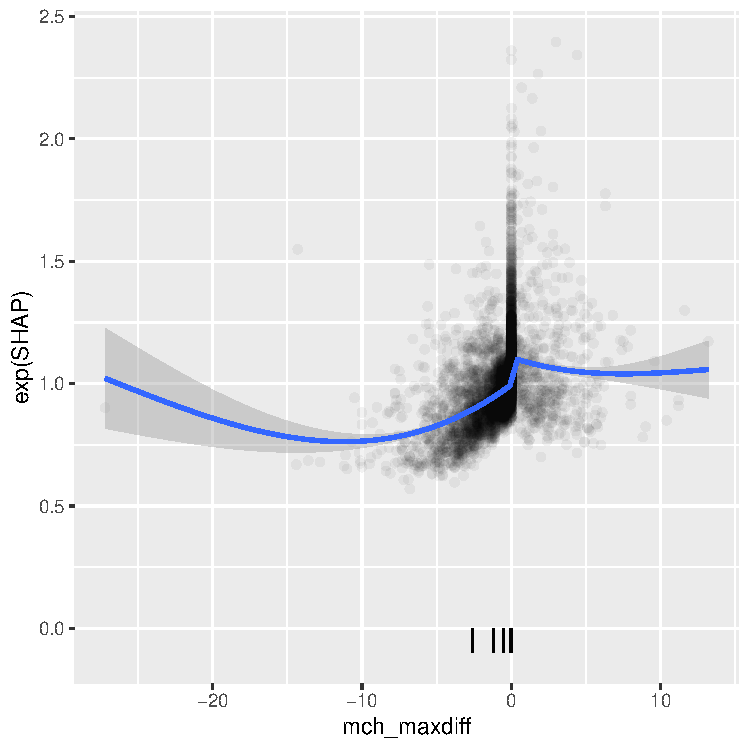
\includegraphics[width=0.49\textwidth]{figures/shap_new/mch_maxdiff.pdf}
%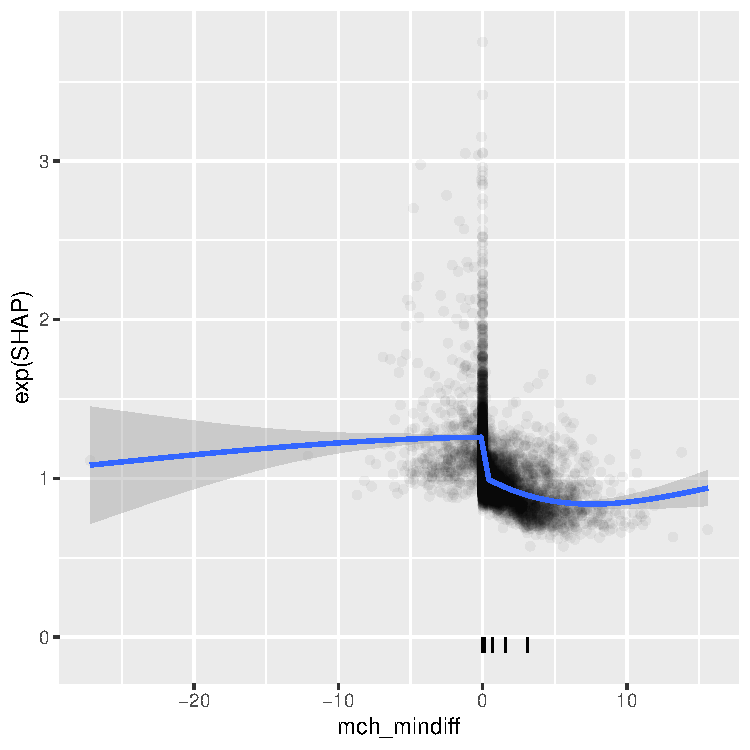
\includegraphics[width=0.49\textwidth]{figures/shap_new/mch_mindiff.pdf}
%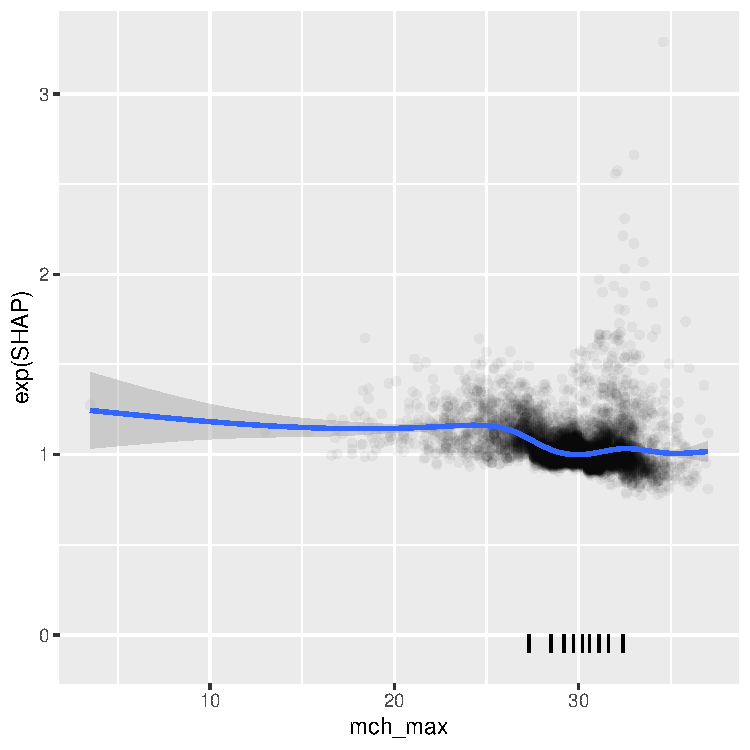
\includegraphics[width=0.49\textwidth]{figures/shap_new/mch_max.pdf}
%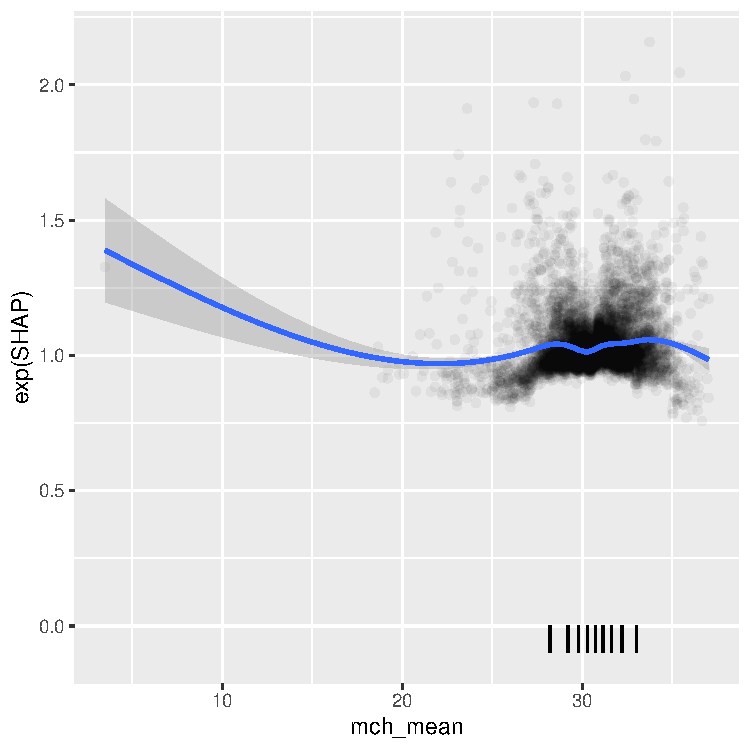
\includegraphics[width=0.49\textwidth]{figures/shap_new/mch_mean.pdf}
%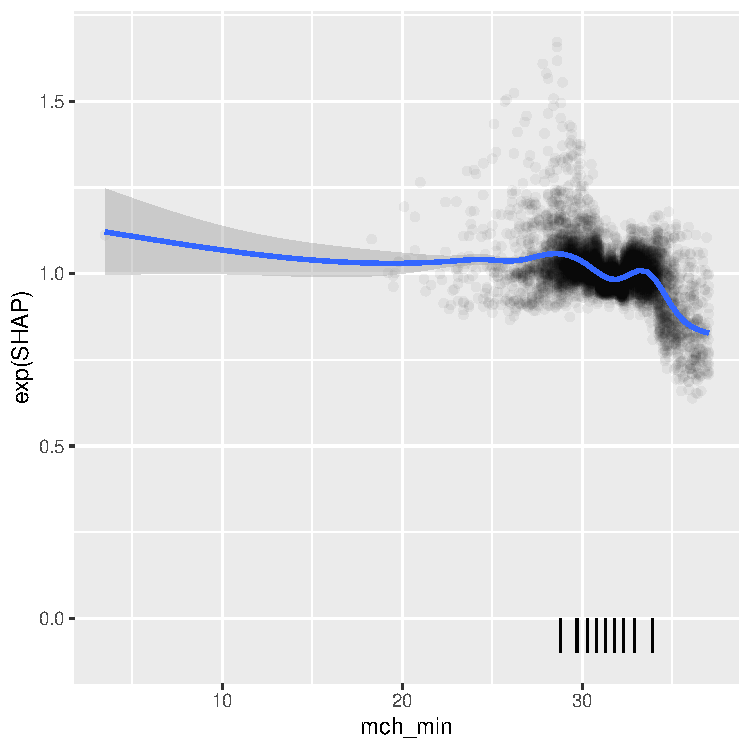
\includegraphics[width=0.49\textwidth]{figures/shap_new/mch_min.pdf}
%\caption{Very negative mindiff(maxdiff) means there is at least one large drop. 
%Very positive maxdiff (mindiff) means at least one large positive jump.
%Small max (min) means always small. Large min (max) means always large.}
%\end{figure}
%
%\begin{figure}[h]
%\centering
%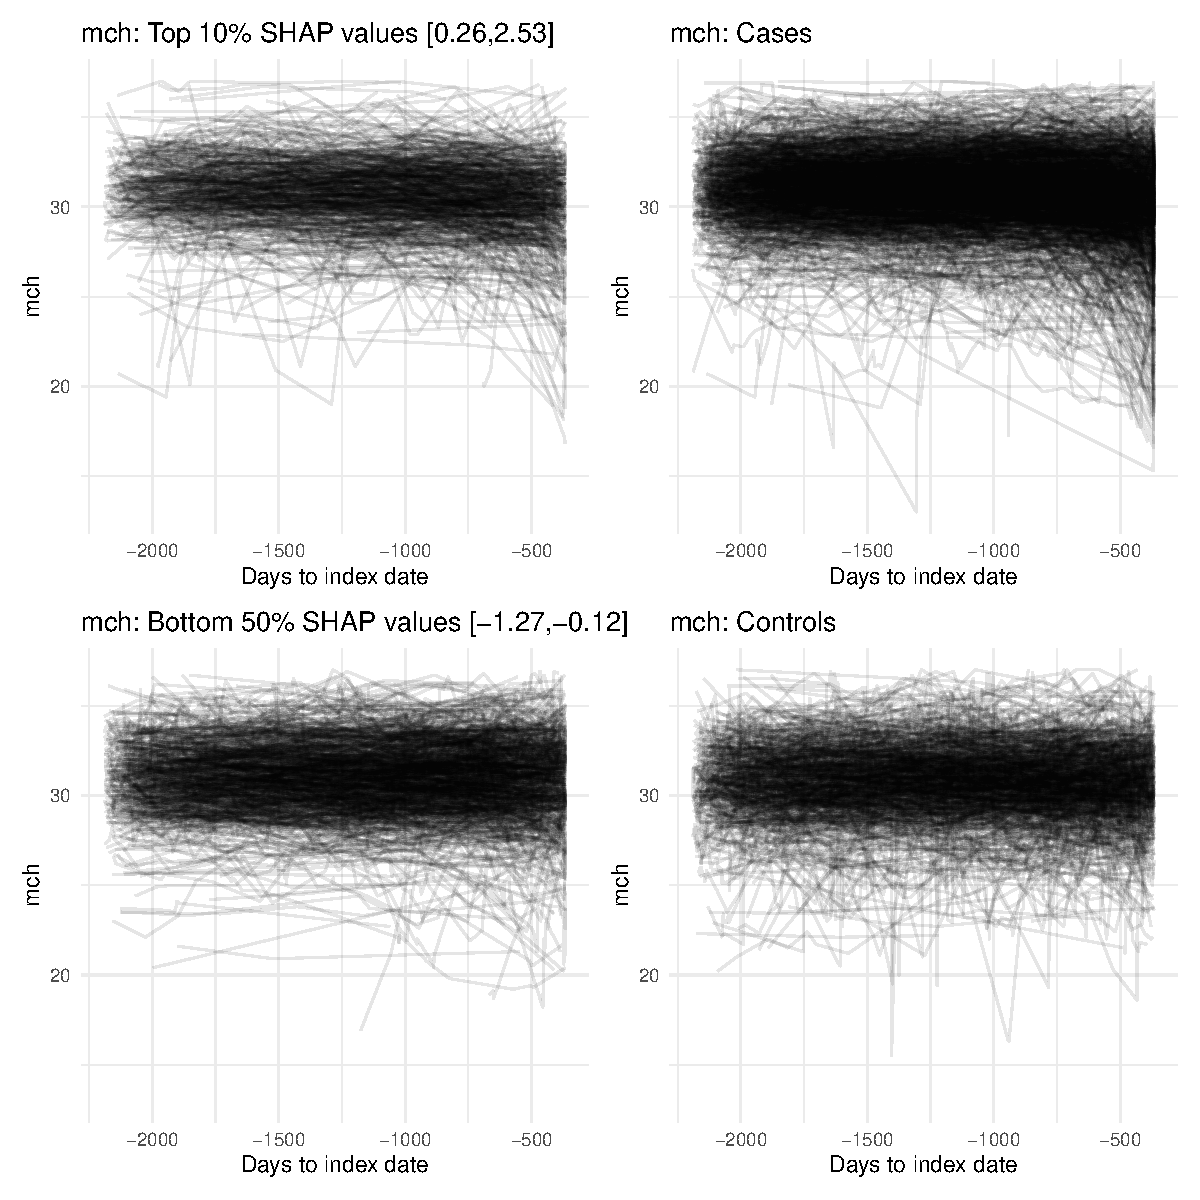
\includegraphics[width=1.0\textwidth]{figures/lab/mch.pdf}
%\caption{Sample of trajectories of mch lab results. Left: stratified by their aggregated SHAP values. Right: straified by case/control status. 
%It is not obvious why some time series have low/high SHAP values just by looking at this, but we at least see that drop towards the end seem
%to be well separated.}
%\end{figure}
%
%\begin{figure}[h]
%\centering
%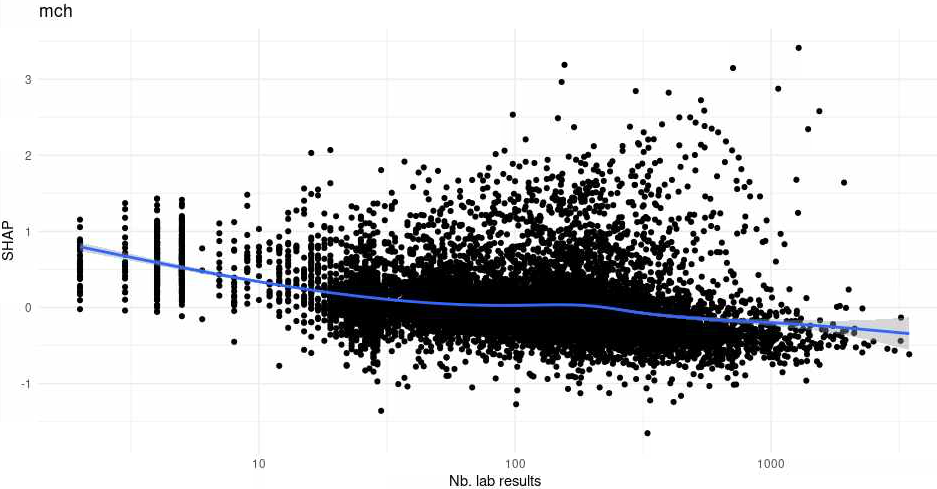
\includegraphics[width=1.0\textwidth]{figures/n_mch.png}
%\caption{It seems that patients with very few lab results indeed have higher predicted risk due to \texttt{mch}.}
%\end{figure}




\clearpage

\section*{Years prior}



\begin{figure}[h]
\centering
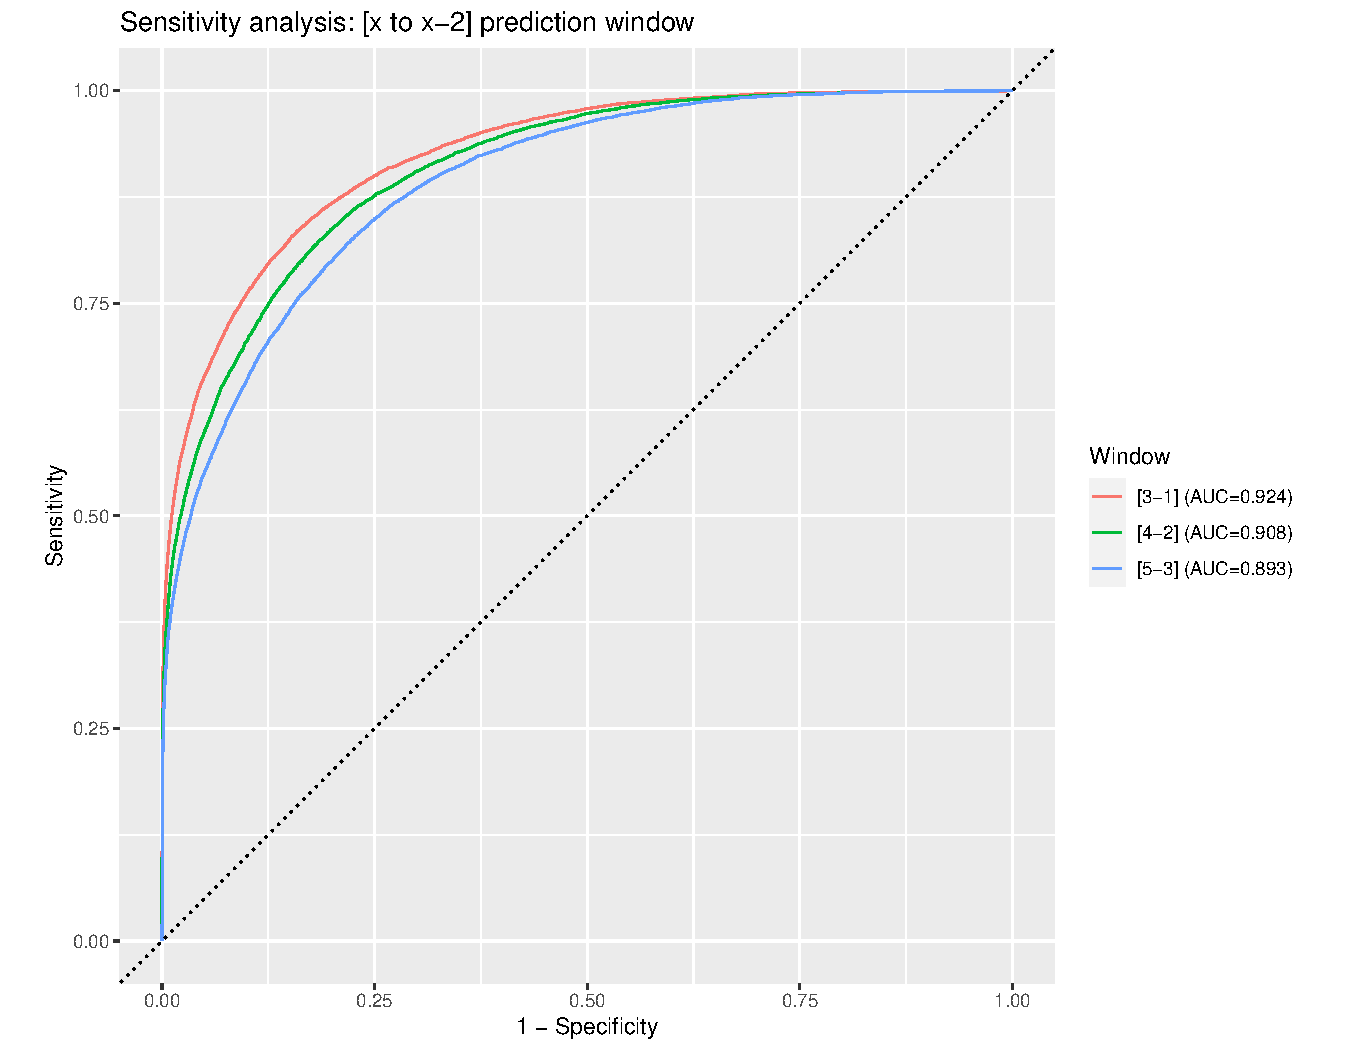
\includegraphics[width=1.0\textwidth]{figures/roc_window_2.pdf}
\caption{In this experiment, all three test set utilizes the same amount of data (2 years), 
but we predict farther in the future (1yr, 2yrs or 3yrs). As expected, we do worse and worse
as we predict further in time, but only by a small margin. This seem to indicate are predictions are 
somewhat valid beyond the 1yr window we used.}
\end{figure}



\begin{figure}[h]
\centering
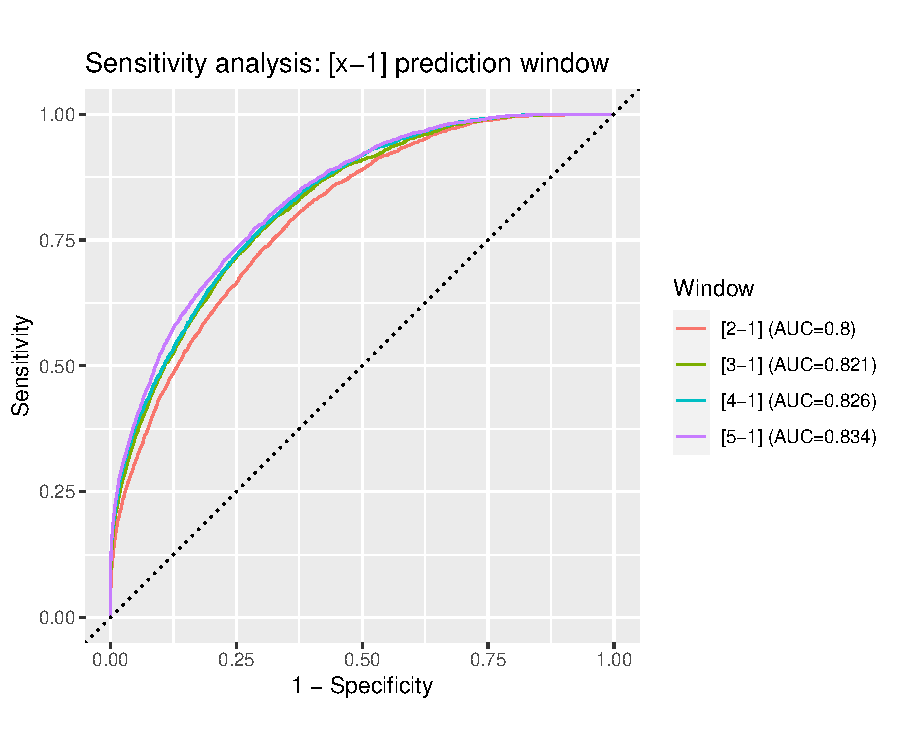
\includegraphics[width=1.0\textwidth]{figures/roc_window_x-1.pdf}
\caption{In this experiment, we decrease the amount of data (from 4yrs to 1yr) in the test set, 
but keep the prediction horizon to 1yr. As expected, performance decreases as the number of years
decrease (we have less and less data). However, we notice a large jump in performance from
3yrs to 4yrs. A possible explanation is that our model is specifically trained for 4 years of data
and the summary features change significantly. In particular, minimum and maximum statistics are 
highly sensitive to having more data. This also increases the amount of missing data.}
\end{figure}



\clearpage
\section*{EAC v EGJAC}

\begin{itemize}
	\item They have different predicted risk
	\begin{itemize}
		\item EGJAC have higher predicted risk, 
		much better separation from controls
		\item Esp. for the region of interest, EAC has a lot more subject around the threshold
	\end{itemize}
	\item Previous comparison of feature distribution was incorrect (was done after imputation)
	\begin{itemize}
		\item see new results below
	\end{itemize}
	\item There is a stark difference in proportion of missing values between EAC and EGJAC cases
	for HCT, LYMPH and MCH. 
	\begin{itemize}
		\item Almost always missing for EGJAC
	\end{itemize}
	\item Some feature have different impact between the two models; EAC is generally very similar to ANY
\end{itemize}


\begin{figure}[h]
\centering
\includegraphics[width=1.0\textwidth]{figures/eac_v_egjac/risk_scatter.pdf}
\caption{Scatter plots of (log) predicted risk by all three models stratified by 
case/control status (none, EAC, EGJAC). We have very strong correlation between EAC and ANY, but
much less between ANY and EGJAC. There is no correlation between EAC and EGJAC for EGJAC patients. 
EGJAC assigns very high predicted risk to EGJAC patients compared to what ANY/EAC does to 
their respective targets.}
\end{figure}

\begin{figure}[h]
\centering
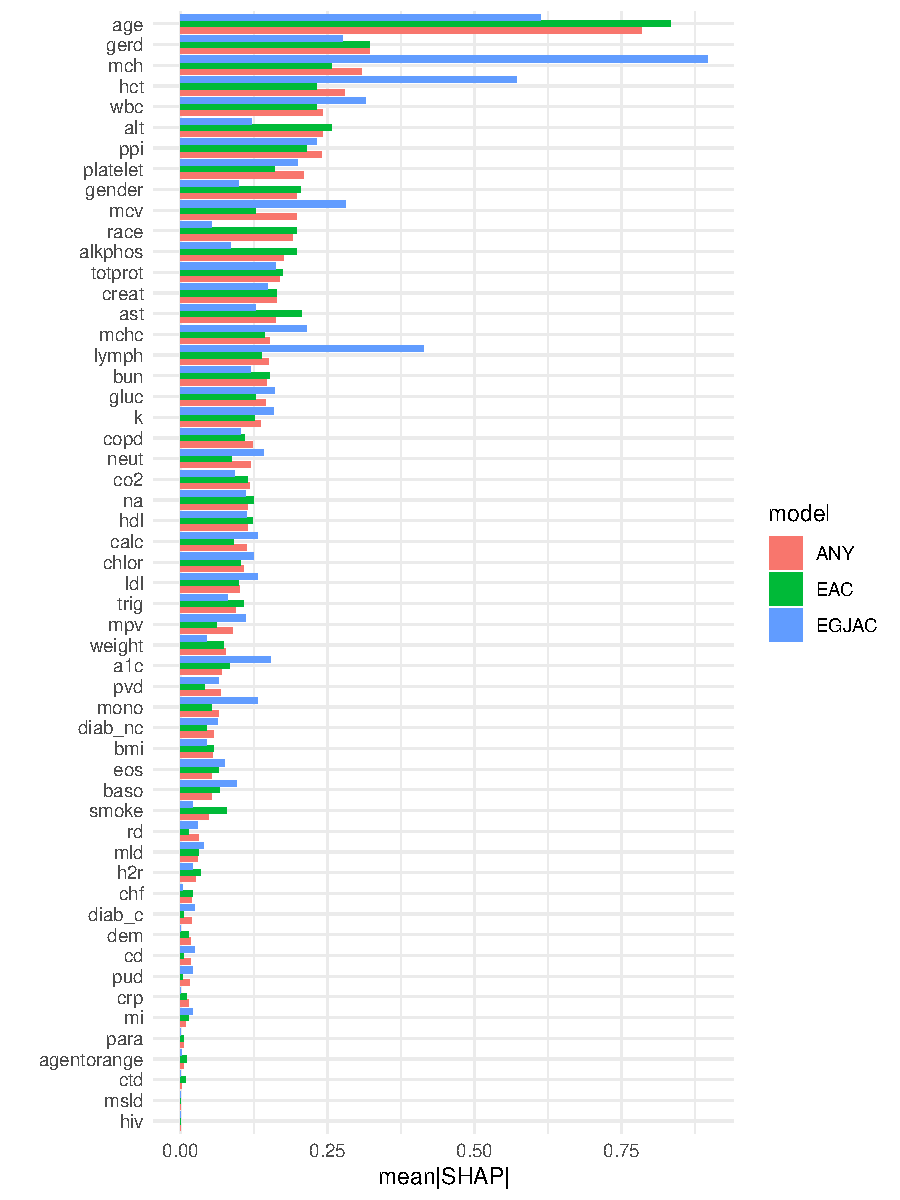
\includegraphics[width=1.0\textwidth]{figures/eac_v_egjac/shap_groups_cancertype.pdf}
\caption{SHAP variable importance wihtin all three models. Notably, we see large differences
\texttt{age}, \texttt{mch}, \texttt{hct}, \texttt{mcv}, \texttt{lymph}, \texttt{race} and a few others.}
\end{figure}


\begin{figure}[h]
\centering
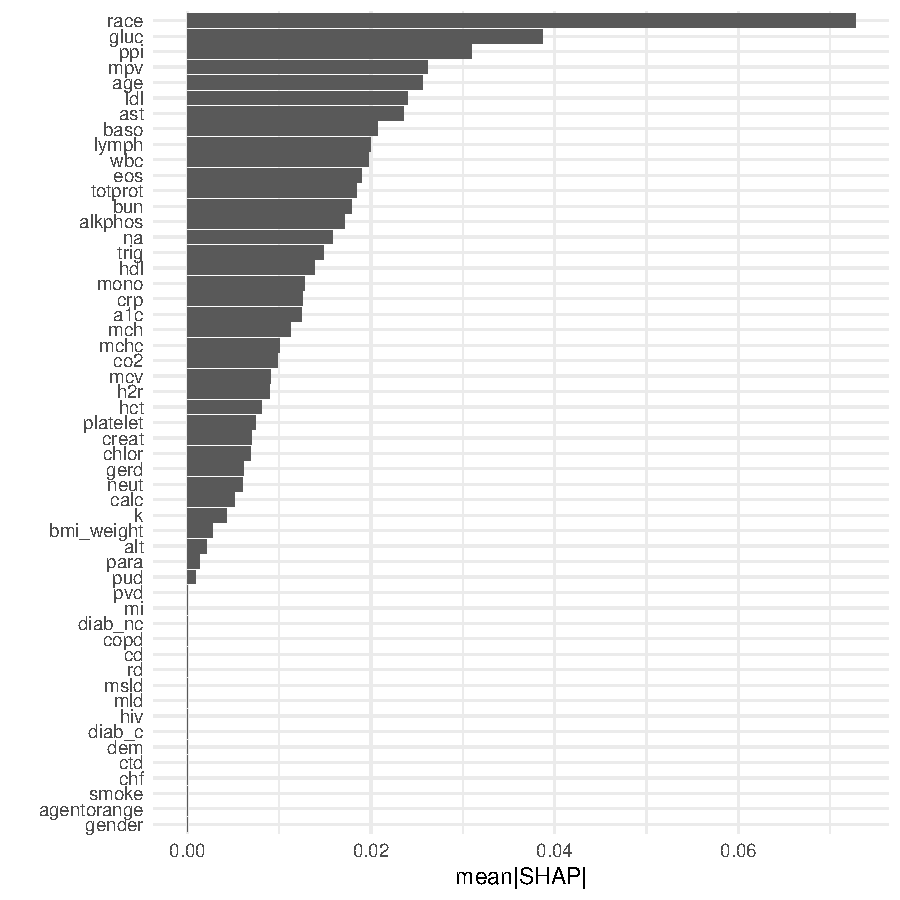
\includegraphics[width=1.0\textwidth]{figures/eac_v_egjac/vs_shap_groups.pdf}
\caption{SHAP variable importance for a model differentiating EAC from EGJAC. We
again find \texttt{mch}, \texttt{hct}, \texttt{mcv}, \texttt{lymph} and \texttt{mchc} at the top}
\end{figure}




\begin{table}[ht]
\centering
\begin{tabular}{lrrrr}
\hline
& Mean (control) & Mean (EAC) & Mean (EGJAC) & pvalue.adj \\
\hline
black & 0.169 & 0.041 & 0.089 & 0.001 \\ 
  gerd & 0.232 & 0.357 & 0.269 & 0.005 \\ 
  baso\_max & 1.017 & 0.328 & 1.791 & 0.033 \\ 
\hline
\end{tabular}
\caption{Features with different means between EAC and EGJAC (at 5\% level, BH). It appears that race and GERD are less important for EGJAC. 
We also find that baso could be different between the two.}
\end{table}





\begin{table}[ht]
\centering
\begin{tabular}{lrrrr}
\hline
& Prop. Control & Prop. EAC & Prop. EGJAC & pvalue.adj \\
\hline

\hline
\end{tabular}
\caption{Features with different proportions of non-NAs between EAC and EGJAC (at 5\% level, BH).
There are None!}
\end{table}


\begin{figure}[h]
\centering
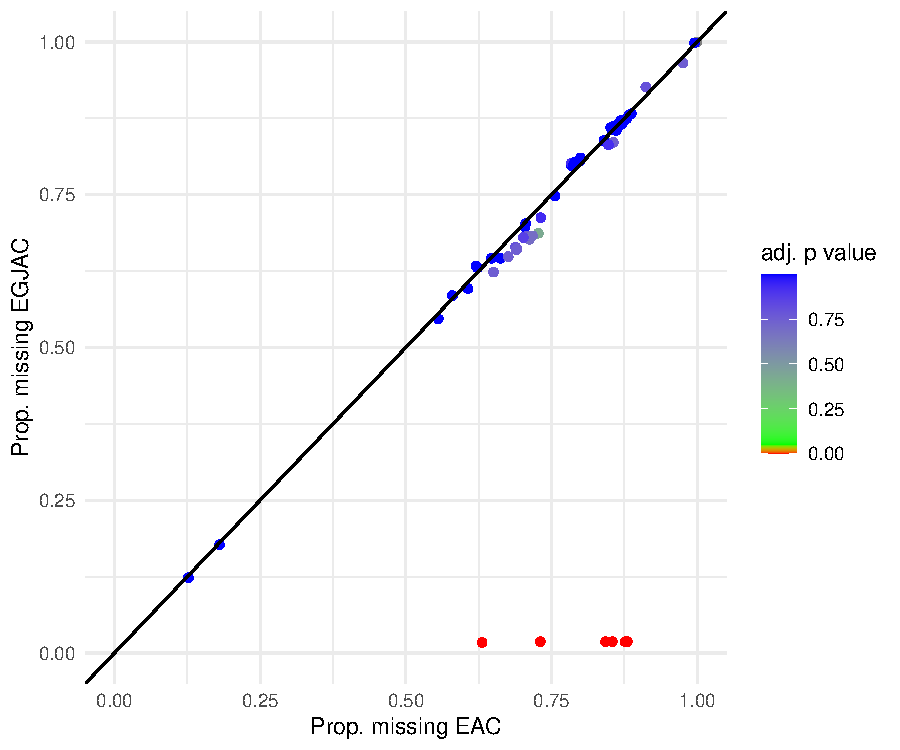
\includegraphics[width=1.0\textwidth]{figures/eac_v_egjac/vs_propNA.pdf}
\caption{Labels are wrong and should read ``non-missing.'' This shows it really is just there three 
that have different missing proportions.}
\end{figure}



\clearpage
\section*{Birth cohort effect}







\clearpage


\section*{***Old stuff to update from here***}
\section*{Feature selection}


\textbf{Correlation}:

\begin{figure}[h]
\centering
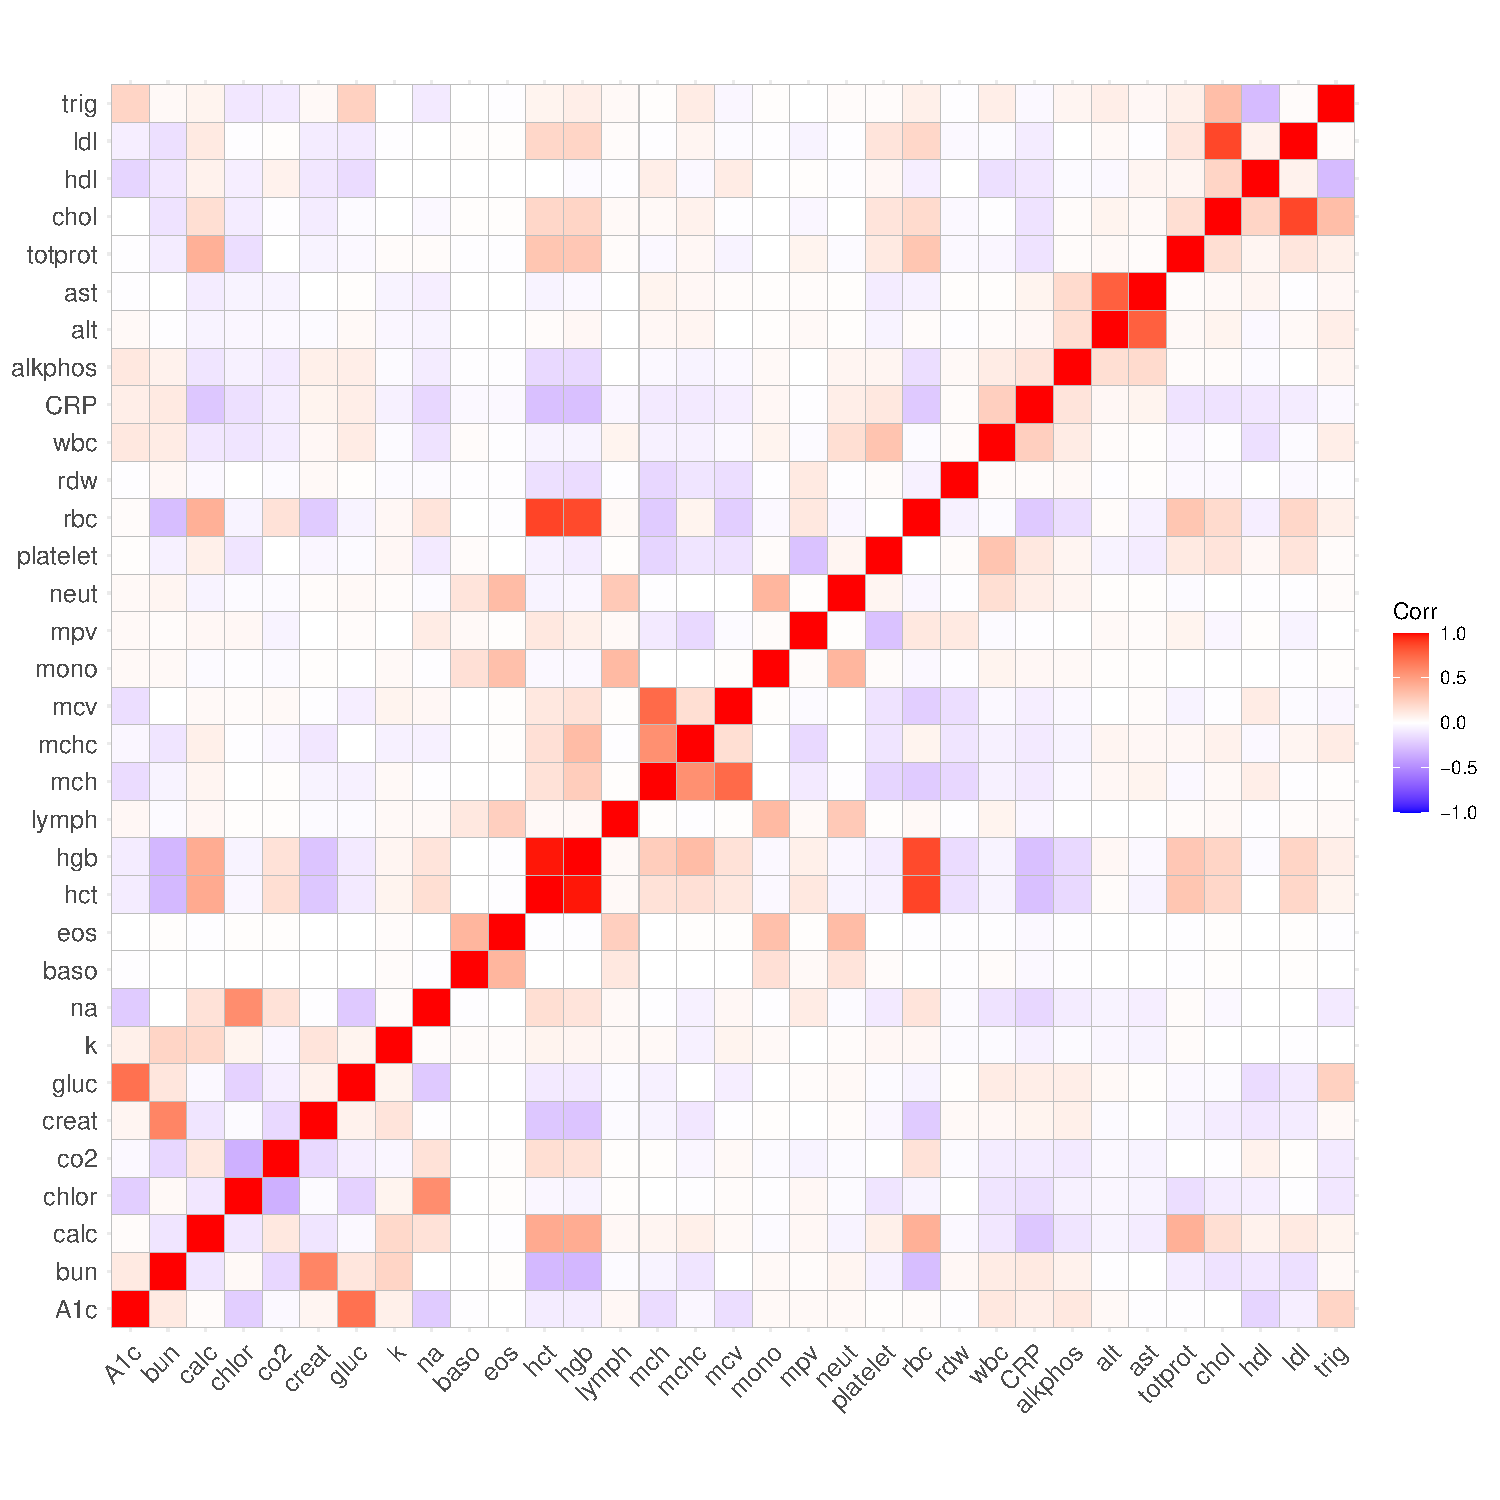
\includegraphics[width=\textwidth]{figures/lab_corr.pdf}
\end{figure}

\begin{table}[h]
\centering
\begin{tabular}{rllr}
  \hline
 & var1 & var2 & correlation \\ 
  \hline
  2 & mchc & mch & 0.569 \\ 
  3 & chlor & na & 0.578 \\ 
  6 & creat & bun & 0.617 \\ 
  8 & gluc & A1c & 0.707 \\ 
  10 & mcv & mch & 0.742 \\ 
  11 & alt & ast & 0.782 \\ 
  13 & hgb & rbc & 0.857 \\ 
  15 & chol & ldl & 0.875 \\ 
  18 & rbc & hct & 0.884 \\ 
  20 & hgb & hct & 0.976 \\ 
   \hline
\end{tabular}
\caption{HGB and HCT are indeed very highly correlated}
\end{table}

\clearpage
\textbf{On chol/ldl/hdl}:
Missingness patterns does not help
\begin{table}[h]
\centering
\begin{tabular}{lrrrrrrrr}
\toprule
Pattern (chol,hdl,ldl) & 000 & 001 & 010 & 011 & 100 & 101 & 110 & 111 \\
\midrule
Prop (\%) & 59.5 & 0.7 & 0.5 & 0.6 & 0.2 & 0.0 & 0.2 & 38.3\\
\bottomrule
\end{tabular}
\end{table}

\textbf{Using performance}:
\begin{itemize}
\item Drop various features:
\begin{itemize}
	\item (colonoscopy, fobt)
	\item two of (hct, hgb, rct)
	\item one or two of (chol, ldl, hdl)
\end{itemize}
\item Refit with 1M controls \& evaluate
\item Proposed is dropping (colonoscopy, fobt, hbg, rct, chol)
\item Conclusions:
\begin{itemize}
	\item Not much difference
	\item Probably best to avoid dropping hct
\end{itemize}
\end{itemize}


\begin{table}[ht]
\centering
\begin{tabular}{lrr}
\toprule
Drop & Valid. AUC & Test AUC \\
\midrule
None & 0.832 & 0.827 \\ \addlinespace
Colonoscopy, fobt & 0.830 & 0.826 \\ \addlinespace
rct, hgb & 0.831 & 0.826 \\
rbc, hct & 0.824 & 0.821 \\
hct, hgb & 0.824 & 0.826 \\ \addlinespace
chol & 0.834 & 0.831 \\
ldl & 0.831 & 0.829 \\
hdl & 0.832 & 0.825 \\
hdl, ldl & 0.831 & 0.830 \\ \addlinespace
(proposed) & 0.827 & 0.827 \\
\bottomrule
\end{tabular}
\end{table}




\end{document}
